\documentclass[fontsize=11pt,
		 %twoside, 
		 oneside,
		 ngerman,
		 titlepage,
		 paper=a4,
		 bibliography=totoc,
		 listof=totoc,
		 DIV=10,
		 BCOR=5mm,
		 headsepline,
		 footsepline,
		 ]{scrartcl}
		 
%% 8-Bit-Standard Font (Cork-Kodierung)
\usepackage[T1]{fontenc} % 256 Zeichen Fonttabelle, statt 128 Zeichen
%% Direkte Eingabe von Umlauten
\usepackage[utf8]{inputenc}
%% Verwendung der neuen deutschen Rechtschreibung

\usepackage[ngerman]{babel} % babel etwas mehr gewartet, moderner
%
\usepackage{scrhack}
%% Kein Einzug am Absatzbeginn
\setlength{\parindent}{0mm}
%
%% Einbinden von Bildern
\usepackage{setspace}
\usepackage{graphicx}
\usepackage{epstopdf}
\usepackage[absolute]{textpos}
\usepackage{geometry}
\usepackage{multirow}
\usepackage{booktabs} % schöne Tabellenabstände und Linien
\usepackage{textcomp} % griechische/spezielle Buchstaben im Text
%
\usepackage[numbers]{natbib} %mit nummer zitieren
\usepackage[cmyk,table]{xcolor}

\usepackage{acronym}
\usepackage{pdfpages}
\usepackage{color}
\usepackage{listings}

\usepackage{wrapfig}

\usepackage{amsmath} % Zentrierte Formeln

\usepackage{float}   % Bilder besser setzen



\usepackage{url}	 % Längere URL für bibtex
\def\UrlBreaks{\do\/\do-}


%\lstset{numbers=left,numberstyle=\tiny,numbersep=5pt}
\lstset{language = C++}
\lstset{language=C++,
                basicstyle=\fontsize{9}{13}\selectfont\ttfamily,
				emph={uint8_t,uint16_t},
				emphstyle={\color{blue}},
                keywordstyle=\color{blue}\ttfamily,
                stringstyle=\color{red}\ttfamily,
                commentstyle=\color{green}\ttfamily,
                morecomment=[l][\color{magenta}]{\#}
}

%

\usepackage[
pdftitle={Bachelorarbeit Entwicklung robuster Übertragung sensibler Messwerte},%
pdfsubject={Bachelorarbeit},%
pdfauthor={Julius Bartel},%
%pdfkeywords={{tudienssemester}, {Stichwort 2 der Arbeit}, {Stichwort 3 der Arbeit}},%
%pdfpagelayout=TwoPageRight,%
plainpages=false,%
pdfpagelabels,%
]{hyperref}
\usepackage[nameinlink]{cleveref} % noabbrev % umfangreicher als varioref % intelligente Querverweise
\crefname{subsection}{Kapitel}{Kapitel}
\crefname{subsubsection}{Kapitel}{Kapitel}
%

%Kopf und Fusszeile
\setlength{\headheight}{2cm}
\setlength{\footheight}{1cm}
\usepackage[automark]{scrlayer-scrpage}
%\usepackage{scrpage2}
\clearscrheadfoot
\pagestyle{scrheadings}
\automark[section]{section}
%\ihead[]{
\includegraphics[width=0.2\textwidth]{Bilder/hm_4C_L_1-4.eps}}	
%\ohead[]{Entwicklung eines IoT-Gateways\\
%19. Oktober 2020
%}	%[fuer plain configuration]{fuer scrheadings configuration}
%\chead[]{}	%[fuer plain configuration]{fuer scrheadings configuration}
%\ifoot[]{Julius Bartel}	%[fuer plain configuration]{fuer scrheadings configuration}
\cfoot[]{\pagemark}	%[fuer plain configuration]{fuer scrheadings configuration}
%\cfoot[]{}	%[fuer plain configuration]{fuer scrheadings configuration}

\usepackage[hang]{caption}
\usepackage[format=hang,justification=centering,singlelinecheck=false]{caption}
\clearcaptionsetup{figure}
\captionsetup[figure]{font=small,format=hang,justification=centerlast, singlelinecheck=true}
\clearcaptionsetup{table}
\captionsetup[table]{font=small,format=hang,justification=centerlast, singlelinecheck=true}



\usepackage{pgfplots}
\pgfplotsset{
  compat=1.11, %moves axis labels near ticklabels (respects tick label widths)
  grid style={dashed},
  %every linear axis/.append style={
  	%		mark = none, %Seite 161 in der Dokuemntation
 	%		smooth, 
 	%		thick},
 }

\usepackage{subcaption}

\begin{document}
\pagenumbering{arabic}
\begin{titlepage}
\thispagestyle{empty}
%Keine Seitenzahlnummerierung
\begin{center}

%\vspace*{0.5cm}

\begin{figure}[h]
    \centering
        
       
\includegraphics[width=0.6\textwidth]{Pictures/hm_4C_L_1-4.eps}
    
 \end{figure}

% \begin{huge}
%    Hochschule Mannheim
%\end{huge}

%\bigskip



\vspace*{2.5cm}
\begin{LARGE}
\textbf{Julius Bartel}
\end{LARGE}

\bigskip

\begin{Huge} 
\textbf{Entwicklung robuster Übertragung sensibler Messwerte}
\end{Huge}


\par\bigskip

\begin{large}
    \textbf{Bachelorarbeit}
\end{large}

\vspace{12cm}
Sommersemester 2021 Betreuer: Prof. Dr.-Ing. Dennis Trebbels




\end{center}

\end{titlepage}

\cleardoublepage

\section*{Selbstständigkeitserklärung}
\addcontentsline{toc}{section}{Selbstständigkeitserklärung}

Hiermit erkläre ich, dass ich die vorliegende Arbeit selbstständig verfasst und keine anderen als die angegebenen Quellen und Hilfsmittel benutzt habe.\vspace{2cm}

$\overline{\mbox{Ort, Datum}~~~~~~~~~~~~~~}$ \hfill $\overline{\mbox{Unterschrift}~~~~~~~~~~~~~~~~~~}$
 \hspace{2cm}
\section*{Zusammenfassung}

\addcontentsline{toc}{section}{Zusammenfassung}


Thema dieser Arbeit ist die Entwicklung einer robusten Kommunikation zwischen zwei \acp{uC} zur Weiterleitung von sensiblen Messdaten und 
der anschließenden Weiterleitung der Daten an ein übergeordnetes Netzwerk. Die Entwicklung soll an Hand eines Praxisbeispiels demonstriert werden.

\smallskip

Grundlage der Arbeit ist meine vorhergegangene Studienarbeit \citep{IoTGateway}, in welcher die Hardware,
welche die Grundlage für dieses Projekt bildet, entwickelt, bestückt und in Betrieb genommen wurde.

Die entwickelte Platine verfügt über zwei \acs{uC}, deren \acs{UART}-Schnittstellen miteinander verbunden sind. Ein Prozessor ist hierbei
für die Verarbeitung von Sensormesswerten zuständig, während der andere als \acs{WLAN}-Relais an ein übergeordnetes Netzwerk fungiert.

\smallskip

Auf Basis der \acs{UART}-Schnittstellen der beiden Prozessoren soll ein Protokoll implementiert werden, welches sowohl den Transport
von Messwerten in die eine Richtung, als auch den Transport von Konfigurationsbefehlen in die andere Richtung ermöglicht. 

Als Praxisbeispiel wurde die kapazitive Messung von Feuchtigkeit im Erdreich gewählt. Die gemessenen Daten sollen verarbeitet und
per \ac{MQTT} an ein Netzwerk weitergeleitet werden.

\smallskip

Der gesamte Code ist in einer GitHub-Repository zu finden \citep{Listing}.
\section*{Abkuerzungsverzeichnis}

\begin{acronym}
    \acro{HAL}{Hardware Abstraction Layer}
    \acro{IoT}{Internet of Things \textit{en. Internet der Dinge}}
    \acro{uC}[\textmu C]{Microcontroller}
    \acro{WLAN}{Wireless Local Area Network \textit{en. Drahtlose Netzwerkverbindung}}
    \acro{RAM}{Random Access Memory}
    \acro{ADC}{Analog Digital Convert \textit{en. Analog-Digital Wandler}}
    \acro{JTAG}{Joint Test Action Group}
    \acro{UART}{Universal Asynchronous Receiver Transmitter}
    \acro{USART}{Uinversal Synchronous Receiver Transmitter}
    \acro{USB}{Universal Serial Bus}
    \acro{MQTT}{Message Queuing Telemetry Transport}
    \acro{SPI}{Serial Periphal Interface}
    \acro{I2C}{Inter-Integrated Circuit}
    \acro{DMA}{Direct Memory Access}
    \acro{AHB-Bus}{Advanced High-Perfomance Bus}
    \acro{GPIO}{General Purpose Input Output}
    \acro{MSB}{Most Significant Bit}
    \acro{LSB}{Least Significant Bit}
    \acro{FIFO}{First In First Out}
    \acro{ASCII}{American Standard Code for Information Interchange}

\end{acronym}

\tableofcontents
\clearpage

\section{Einführung}
\label{sec:Einführung}





\subsection{Vorhergegangene Arbeit}



\begin{wrapfigure}{l}{0.45\textwidth}
    % \begin{figure}[h]
     \vspace{-\baselineskip}
         \centering
         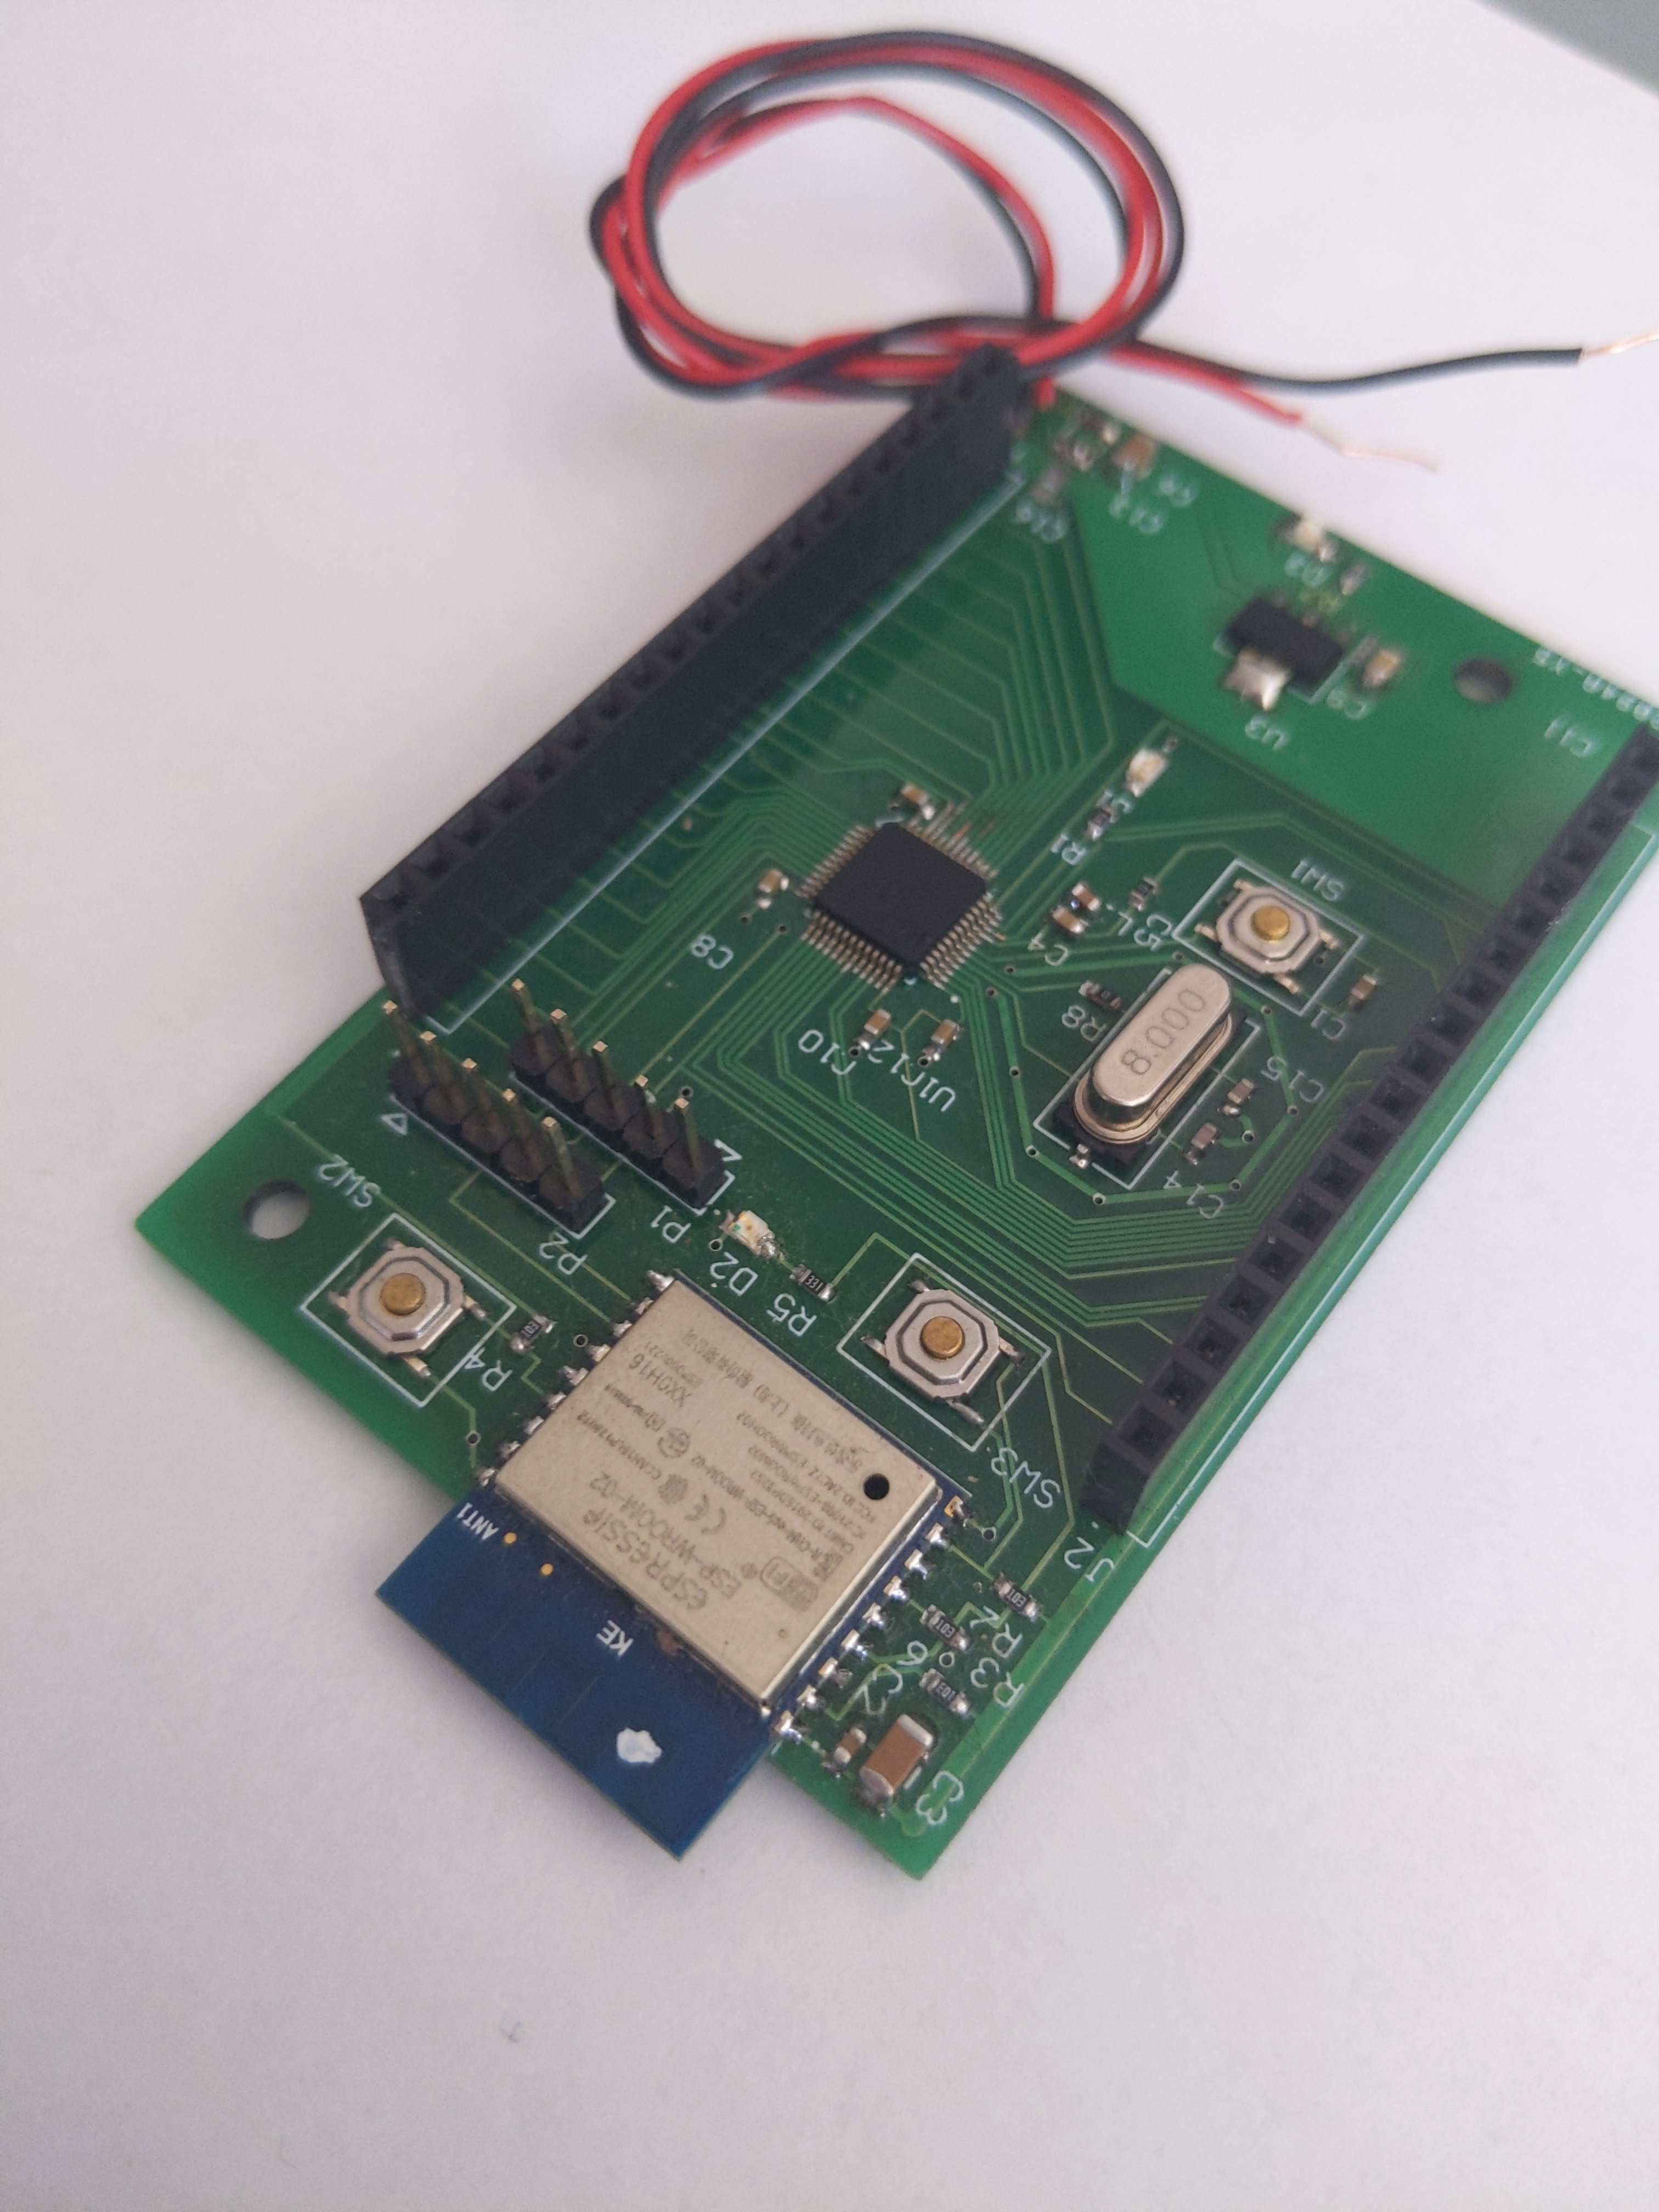
\includegraphics[scale=0.05]{Pictures/assembled.jpg}
         \caption{\textit{IoT-Gateway \citep{IoTGateway}}}
         \label{img:IoT-Gateway}
    % \end{figure}
 \end{wrapfigure}

In der vorhergegangenen Arbeit (\textit{Entwicklung eines IoT-Gateways \citep{IoTGateway}}) wurde eine Platine, zu sehen in Abb. \ref{img:IoT-Gateway}, 
entwickelt, welche die Grundlage der vorliegenden Arbeit bildet. 

\smallskip


Die Platine verfügt über zwei \ac{uC}. Einer der Prozessoren, genauer ein \textit{STM32F103C8}, ist für das Auslesen von Messwerten und die
Verarbeitung dieser zuständig, während der andere Prozessor, ein \textit{ESP8266}, die Netzwerkanbindung per \acs{WLAN} ermöglicht.

\smallskip

Abgesehen von den beiden Prozessoren verfügt das Board über einen linearen Spannungsregler, um 3.3V für die \acp{uC} bereitzustellen. Des Weiteren
wurden die nötigen externen Beschaltungen für die beiden Prozessoren entwickelt. Beide Prozessoren verfügen über Status-LEDs. 
Die \acs{GPIO} des STM32 werden über Buchsenleisten herausgeführt, um den einfachen Anschluss von Erweiterungsplatinen zu ermöglichen.

\smallskip

Die Programmierung des STM32 erfolgt mit Hilfe eines propietären Programmiergeräts (\textit{ST-Link V2}), während der ESP8266 mit Hilfe eines
\acs{UART}-USB Interfaces programmiert wird. 
\subsection{Aufbau der Arbeit}

Diese Arbeit ist in mehrere Abschnitte geteilt:

\begin{itemize}
    \item Erklärung der Grundlagen
    \item Implementation der Funktionen in Software
    \item Test an Hand eines Praxisbeispiels
    \item Auswertung und Fazit sowie Aussicht
\end{itemize}

Im Beginn dieser Arbeit sollen zuerst die Grundlagen erklärt werden, auf denen diese Arbeit aufbaut. Diese spannen von den Eigenschaften
der \ac{uC} über die genutzten Protokolle zu diversen Datenstrukturen und Algorithmen.

Anschließend werden die zuvor besprochenen Grundlagen in Software implementiert um sie dann an Hand eines Praxisbeispiels zu testen.

Zu guter letzt wird die Arbeit ausgewertet, ein Fazit über die Entwicklungen gezogen und eine Aussicht präsentiert, wie das Projekt
weiterentwickelt werden oder verbessert werden kann. 
\clearpage

\section{Grundlagen}
\label{sec:Grundlagen}
\subsection{Microcontroller}

\subsubsection{ESP8266}

\begin{wrapfigure}{r}{0.45\textwidth}
    \vspace{-\baselineskip}
	\centering
	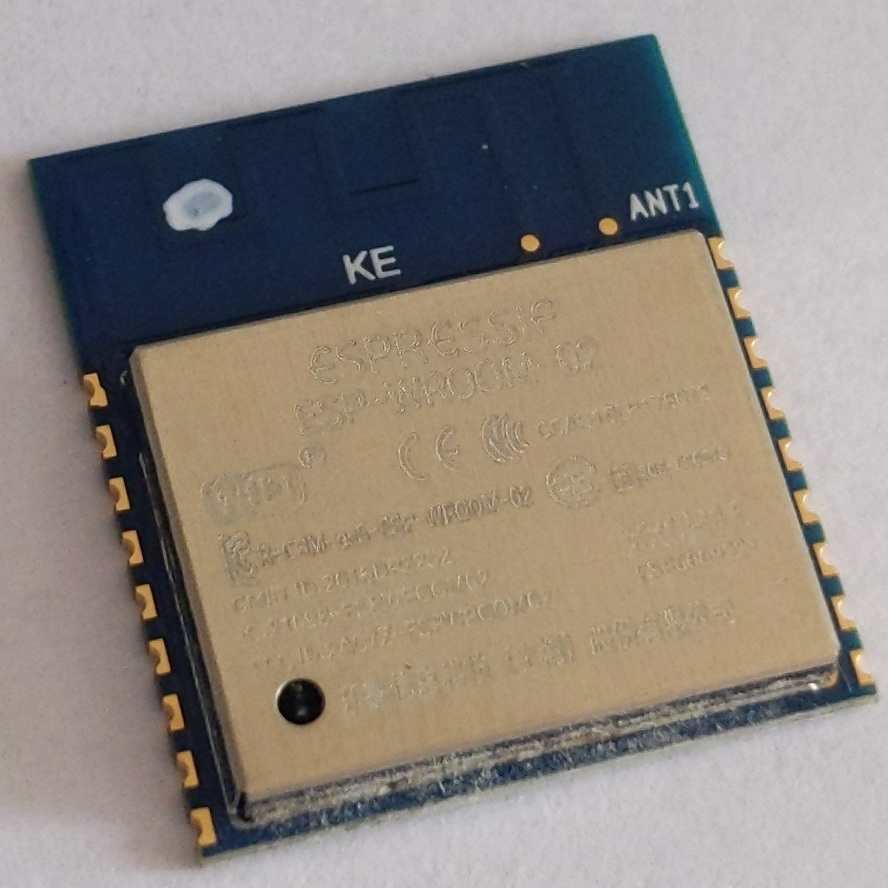
\includegraphics[scale=0.6]{Pictures/esp.jpg}
	\caption{\textit{ESP8266 WROOM-02}}
	\label{img:ESP8266 WROOM-02}
\end{wrapfigure}

Der ESP8266 ist ein 32-Bit \ac{uC} mit einem Systemtakt von 80MHz - 160MHz. Er verfügt über 64kB \ac{RAM} welcher als Arbeitsspeicher genutzt
wird, sowie über 96kB \ac*{RAM} welcher als Datenspeicher genutzt wird. Während des Bootvorgangs wird die Firmware aus einem externen Flashspeicher
geladen. Der \ac{uC} verfügt über alle gängigen Peripherien (\acs{ADC},\acs{UART},\acs{SPI},\acs{I2C}) sowie über eine \acs{WLAN}-Schnittstelle
welche mit dem Standard \textit{802.11 b/g/n} arbeitet und im 2.4-2,5GHz Band kommuniziert \citep{ESP8266_Datasheet}.

\smallskip

In diesem Anwendungsfall wird der ESP8266 als Modul eingesetzt (ESP8266-WROOM-02), da dieses bereits über die nötige externe Beschaltung (Oszillator, Flashspeicher, Antenne)
verfügt \citep{ESP8266_Datasheet}.

\smallskip

Die Programmierung erfolgt über \ac{UART} mittels einem USB-Adapter.

\subsubsection{STM32F103}

Der STM32F103 \ac{uC} basiert auf der Cortex M3 Architektur von ARM und arbeitet mit einem Systemtakt von bis zu 72MHz. Die hier eingesetzte 
Version STM32F103C8 verfügt über 64kB Flashspeicher sowie 20kB \ac{RAM}.

\begin{wrapfigure}{r}{0.45\textwidth}
    % \begin{figure}[h]
     \vspace{-\baselineskip}
         \centering
         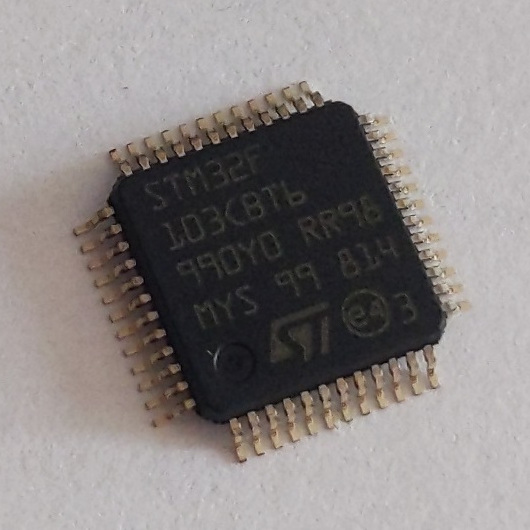
\includegraphics[scale=0.8]{Pictures/stm32f103.jpg}
         \caption{\textit{STM32F103C8}}
         \label{img:STM32F103C8}
    % \end{figure}
 \end{wrapfigure}

\smallskip

An den 37 Ein- und Ausgängen des \acp{uC} sind diverse Kommunikationsschnittstellen verfügbar (CAN,I2C,SPI,USART,USB). 
Desweiteren verfügt der STM32F103 über einen 10-Kanaligen 12-Bit \acs{ADC}, diverse Timer mit verschiedenem Funktionsumfang
sowie über einen \acs{DMA}-Controller. 

\smallskip

Für die Programmierung des \ac{uC} ist ein s.g. ST-Link Programmiergerät notwendig, welches auch Debugging ermöglicht.



\clearpage
\subsection{Peripherie}

Dieser Abschnitt erklärt die verschiedenen genutzten Peripherien. Diese beziehen sich jedoch primär auf die Funktionen des STM32, da diese
dort intensiver Nutzung unterliegen, während die einzigen genutzten Funktionalitäten des ESP8266 seine WLAN und UART Schnittstelle sind,
welche durch das Arduino-Framework verschleiert werden.

\subsubsection{UART/USART}

Der STM32F103 verfügt über drei \acs{USART}-Schnittstellen, welche jedoch auch als \ac{UART} genutzt werden können \citep{STM32_Datasheet}.
Die dabei genutzten Spannungspegel entsprechen hierbei die der TTL-Logik \citep{STM32_Datasheet}.

\smallskip

Die Einheiten verfügen unter anderem auch über Idle-Line Detection (\textit{Erkennung von Kommunikationsstops}), Duplex und Hardware Flow 
Control \citep{STM32_Ref}.




\subsubsection{DMA}

\begin{wrapfigure}{r}{0.35\textwidth}
    % \begin{figure}[h]
     \vspace{-\baselineskip}
         \centering
         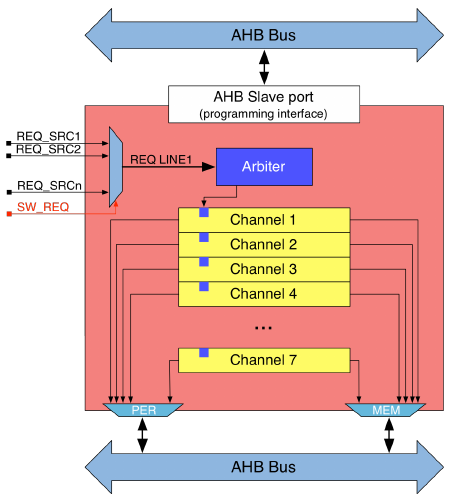
\includegraphics[scale=0.3]{Pictures/dma_channel.png}
         \caption{\textit{DMA \citep{MasteringSTM}}}
         \label{img:DMA_Controller}
    % \end{figure}
 \end{wrapfigure}

Der \acl{DMA} Controller ist eine dedizierte Hardwareeinheit, welche das direkte schreiben von Daten in den Speicher des \ac{uC} erlaubt - ohne, dass dafür Instruktionen durch den Prozessor
ausgeführt werden müssen. Die unterstützen Peripherien sind Timer, \acs{ADC}, \ac{SPI}, \acs{I2C} und \acs{UART} \citep{STM32_Datasheet}.

\smallskip

Es ist möglich, Daten von Speicherort zu Speicherort, von einer Peripherie zu einem Speicherort oder von einem Speicherort zu einer Peripherie
zu transferieren. Der STM32F103 verfügt über sieben \ac{DMA}-Kanäle.

\smallskip

Durch die Nutzung von \ac{DMA} wird der Prozessor entlastet, da dieser somit nicht mit der Übertragung von Daten blockiert wird. Die Daten werden 
über eine interne Busmatrix direkt übertragen \citep{MasteringSTM}.

\smallskip

Abbildung \ref{img:DMA_Controller} zeigt den Aufbau eines einzelnen Controllers. Jeder \ac{DMA}-Controller verfügt über bis zu sieben Kanäle, deren Priorität von s.g. Arbiter verwaltet werden. Der Nutzer kann den verschiedenen Kanälen,
die jeweils mit einer Peripherieeinheit verknüpft werden können, Prioritäten zuweisen. Der \ac{DMA} ist über den s.g. \acs{AHB-Bus} mit den 
Peripherieeinheiten und dem Speicher des \ac{uC} verknüpft \citep{MasteringSTM}.

\smallskip

Des weiteren verfügt der \ac{DMA}-Controller über einen Slave-Port. Mittels dieses Anschlusses lässt sich der \ac{DMA}-Controller konfigurieren \citep{MasteringSTM}.

\newpage

\subsubsection{ADC}

Ein \acl{ADC} ermöglicht die Konversion von analogen Signalen in digitale Werte, um diese dann mittels des \ac{uC} weiterzuverarbeiten. 
Der \ac{ADC} des STM32F103 hat eine Auflösung von 12-Bit bei bis zu 16 Kanälen und arbeitet nach dem Prinzip der sukzessiven Approximation \citep{STM32_Datasheet}.

\smallskip


\begin{figure}[h]
     \vspace{-\baselineskip}
         \centering
         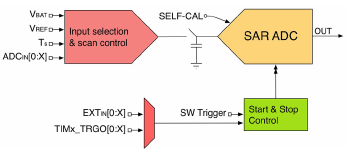
\includegraphics[scale=0.6]{Pictures/adc.png}
         \caption{\textit{Aufbau \citep{MasteringSTM}}}
         \label{img:ADC}
\end{figure}


Es ist möglich, den \ac{ADC} automatisch zu kalibrieren und ihn entweder per Software-Trigger, Timer oder externen Interrupt zu starten. 
In Abbildung \ref{img:ADC} ist der vereinfachte Aufbau des \ac{ADC} abgebildet.

\smallskip 

Des weiteren verfügt der \ac{ADC} über verschiedene Betriebsmodi \citep{STM32_Ref}:
\begin{itemize}
    \item Single Mode 
    \item Continuous Mode
    \item Discontinuous Mode
\end{itemize}

Im Single Mode wird eine Konversion durchgeführt, während im Continuous Mode ständig weitere Konversionen durchgeführt werden. Im Discontinuous Mode
wird die nächste Konversion durchgeführt, sobald ein benutzerdefinierter Trigger ausgelöst wird. Es ist im (Dis-)Continuous Mode möglich, bei 
jeder Konversion einen anderen Kanal des \ac{ADC} anzusprechen.

\newpage

\subsubsection{GPIO}

Der STM32F103 besitzt diverse \acs{GPIO}. Mit Hilfe dieser Ein- und Ausgänge können Signale ein- oder ausgegeben werden. Es ist möglich,
den Anschlüssen interne Pull-Up oder Pull-Down Widerstände zuzuweisen \citep{STM32_Datasheet}. Ausgänge können entweder als Push-Pull oder Open-Drain
konfiguriert werden \citep{STM32_Ref}.

\smallskip

Die Eingänge können,je nach anliegendem Signal, Interrupts auslösen \citep{STM32_Ref}:
\begin{itemize}
    \item Steigende Flanke
    \item Fallende Flanke
    \item Steigende oder Fallende Flanke
\end{itemize}

Die interne Beschaltung der \ac{GPIO} ist Abb. \ref{img:GPIO} zu entnehmen.

\vspace{0.5cm}

\begin{figure}[h]
    \vspace{-\baselineskip}
        \centering
        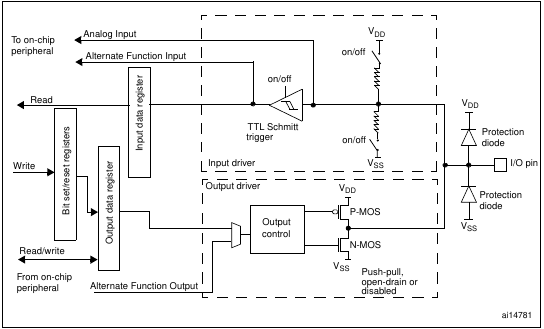
\includegraphics[scale=0.6]{Pictures/gpio.png}
        \caption{\textit{Beschaltung \citep{STM32_Ref}}}
        \label{img:GPIO}
\end{figure}

\newpage


\subsubsection{Timer}

Die Timer des STM32F103 teilen sich, wie in Abb. \ref{img:Timer} zu sehen, in zwei Gruppen auf:

\vspace{0.5cm}
\begin{figure}[h]
    \vspace{-\baselineskip}
        \centering
        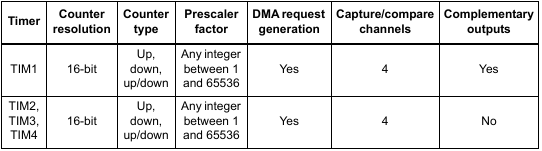
\includegraphics[scale=0.6]{Pictures/timer.png}
        \caption{\textit{Timer \citep{STM32_Datasheet}}}
        \label{img:Timer}
\end{figure}

TIM1 ist ein s.g. Advanced-Control Timer, während TIM2,TIM3 und TIM4 s.g. General-Purpose Timer sind. 

Advanced-Control Timer implementieren erweiterteFunktionen, wie z.B. dreiphasige PWM oder programmierbare Totzeiten\citep{STM32_Datasheet}. 

\smallskip

Abgesehen von den bereits vorgestellten Timern stehen zwei Watchdog-Timer sowie ein s.g. SysTick-Timer zur Verfügung.

Der SysTick-Timer wird einerseits genutzt, um ein Real-Time Operating System auf dem STM32F103 zu realisieren und andererseits um 
dem Hardware Abstraction Layer des STM32F103 eine Zeitkonstante zu geben. Er kann auch als simpler Timer benutzt wird, da er jede
ms aktualisiert wird.

\smallskip

Watchdog-Timer werden genutzt, um abnormale Systemzustände zu erkennen. Ein Beispiel hierfür ist das festhängen in spezifischen Codeabschnitten.




\clearpage
\subsection{Protokolle}
\subsubsection{UART}
\paragraph{Grundlagen}
\subparagraph{Parität}
Das Paritätsbit dient als Ergänzung einer Folge von Bits. Durch das Ergänzen und das entsprechende Setzen des Bits, wird sichergestellt,
dass die Anzahl der Bits gerade ist.

\smallskip

\begin{wrapfigure}{r}{0.3\textwidth}
    % \begin{figure}[h]
     \vspace{-\baselineskip}
         \centering
         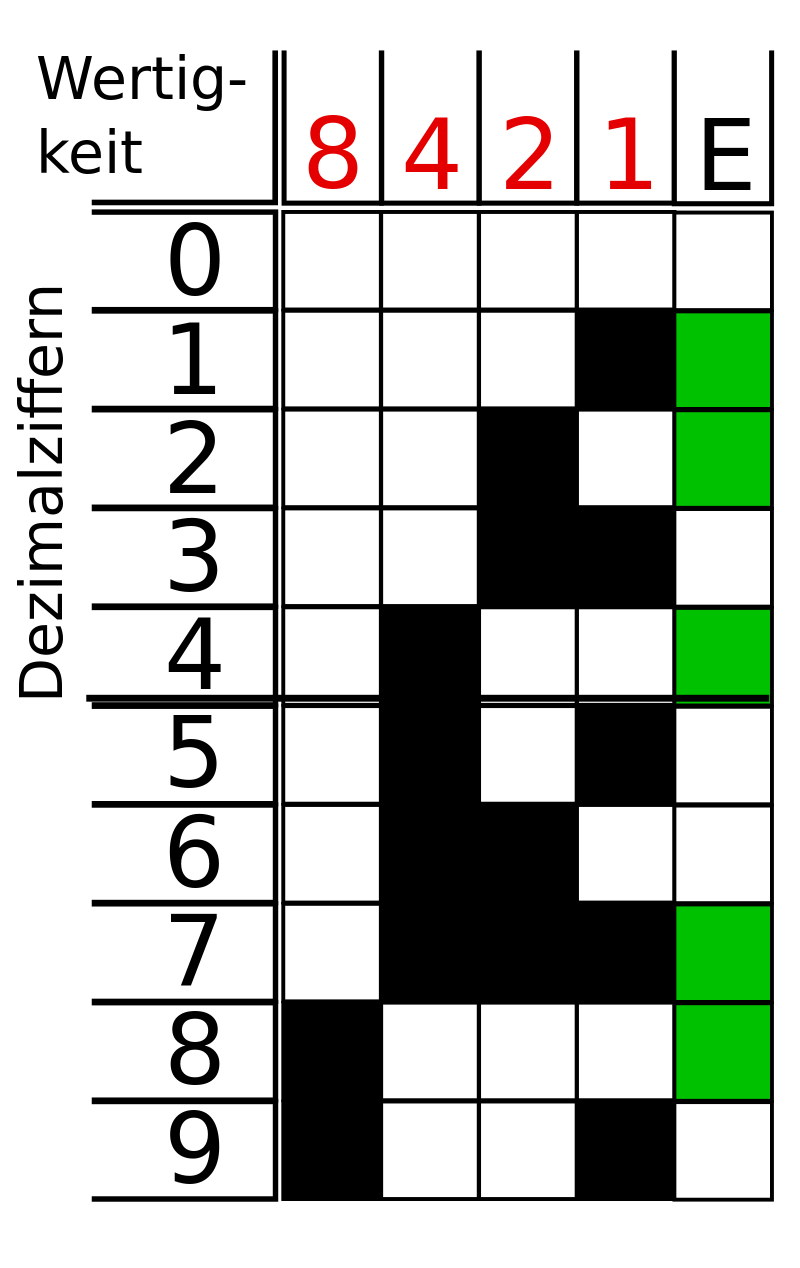
\includegraphics[scale=0.1]{Pictures/paritaet.png}
         \caption{\textit{Parität \citep{ImgParitaet}}}
         \label{img:paritaet}
    % \end{figure}
 \end{wrapfigure}

\smallskip
Die Nutzung eines Paritätsbits ist die einfachste aller Möglichkeiten, Übertragungsfehler zu erkennen. Kippt während der Übertragung eines
der zu übertragenen Bits, ist die Zahl der Bits nicht mehr gerade - ein Fehler liegt vor.

Es ist allerdings nicht möglich festzustellen, wo genau der Fehler aufgetreten ist \citep{Bussysteme}.

\smallskip

Abb. \ref{img:paritaet} zeigt die Applikation eines Paritätsbits bei der binären Repräsentation der Dezimalzahlen eins bis acht. Sobald die Anzahl der 
gesetzten Bits ungerade ist, wird ein Paritätsbit (E) hinzugefügt.

\subparagraph{Baudrate}\label{para:baud}

Die Baudrate, auch Symbolrate genannt, beschreibt die Geschwindigkeit mit der Zeichen übertragen werden.

Ein Baud entspricht hierbei ein Zeichen pro Sekunde \citep{Bussysteme}.

Beispiele für gängige, standarisierte Baudraten für die Übertragung per \ac{UART} sind:

\begin{itemize}
    \item 4800 Baud
    \item 9600 Baud
    \item 115200 Baud
\end{itemize}

Diese Baudraten werden von den meisten Computer- oder Prozessorsystemen unterstützt \citep{Bussysteme}.

\newpage

\paragraph{Erklärung}

Der \acl{UART} ist eine elektronische Schaltung, oder im Falle eines \ac{uC}, eine Peripherieeinheit, welche
die Datenübertragung mit einem anderen System ermöglicht. Die Übertragung läuft hierbei asynchron,
d.h. ohne ein Taktsignal, welches ebenfalls übertragen wird, ab \citep{Bussysteme}. Die Übertragungsgeschwindigkeit
wird in Baud  \ref{para:baud} angegeben.

\smallskip

\begin{wrapfigure}{r}{0.3\textwidth}
    % \begin{figure}[h]
     \vspace{-\baselineskip}
         \centering
         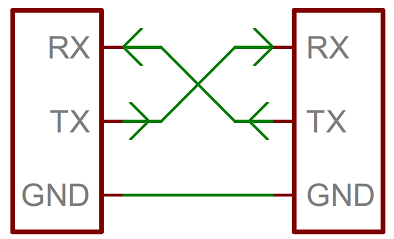
\includegraphics[scale=0.45]{Pictures/uart_rx_tx.png}
         \caption{\textit{Verbindung \citep{ImgRXTX}}}
         \label{img:uart_rxtx}
    % \end{figure}
 \end{wrapfigure}


Jede Seite der Übertragung verfügt über zwei Anschlüsse, \textbf{RX} und \textbf{TX}. \textbf{RX} steht hierbei
für Receiver (\textit{engl. Empfänger}), währen \textbf{TX} für Transmitter (\textit{engl. Sender}) steht.

Für eine korrekte Funktion müssen die beiden Anschlüsse "über Kreuz", wie in Abb. \ref{img:uart_rxtx} dargestellt, verbunden werden \citep{Mikroprozessortechnik}.

\smallskip

Es existieren verschiedene Implementationen von \ac{UART}, welche sich in der Nachrichtenlänge und der Art der
Parität unterscheiden (gerade oder ungerade Parität). Ein oft genutztes Format ist das s.g. \textbf{8N1}-Format.

\smallskip


Die Abkürzung steht hierbei für 8 Bits Nachrichtenlänge und \textit{keine} Parität und ein Stop-Bit. Es wird jedoch neben dem \textit{Stop-}Bit
immer noch ein weiteres Bit übertragen, das \textit{Start-}Bit. Diese zwei Bits repräsentieren das s.g. Framing \textit{engl.: Einrahmen} 
(siehe Abb. \ref{img:uart_framing}) und signalisieren den Beginn und das Ende der Nachricht. Der Beginn einer Nachricht wird mit einem 
Wechsel von '1' auf '0' signalisiert, während das Ende einer Nachricht mit einem Wechsel von '0' auf '1' signalisiert wird \citep{Mikroprozessortechnik}. 

\vspace{0.5cm}

\begin{figure}[h]
    \vspace{-\baselineskip}
        \centering
        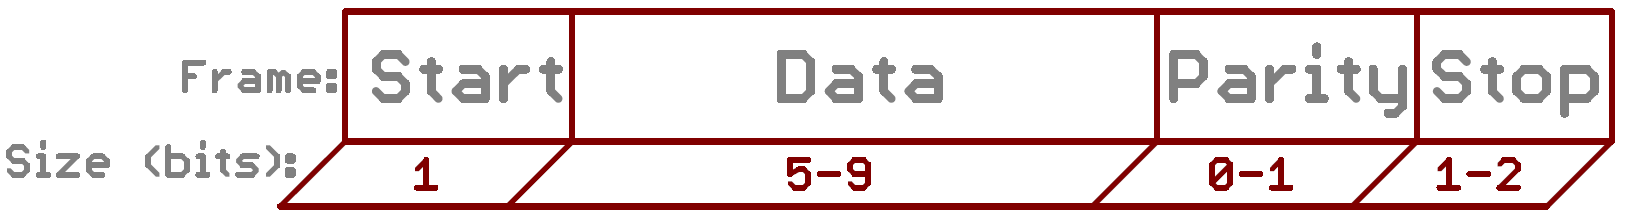
\includegraphics[scale=0.3]{Pictures/uart_framing.png}
        \caption{\textit{Framing \citep{ImgRXTX}}}
        \label{img:uart_framing}
\end{figure}

Sollen nun z.B. die ASCII-Zeichen '\textbf{O}' und '\textbf{K}' im 8N1-Format übertragen werden, 
sähe die Bitreihenfolge wie in Abb. \ref{img:uart_ok} dargestellt aus. Es ist dabei zu beachten, dass das
\acs{LSB} zuerst übertragen wird.

\vspace{0.5cm}

\begin{figure}[h]
    \vspace{-\baselineskip}
        \centering
        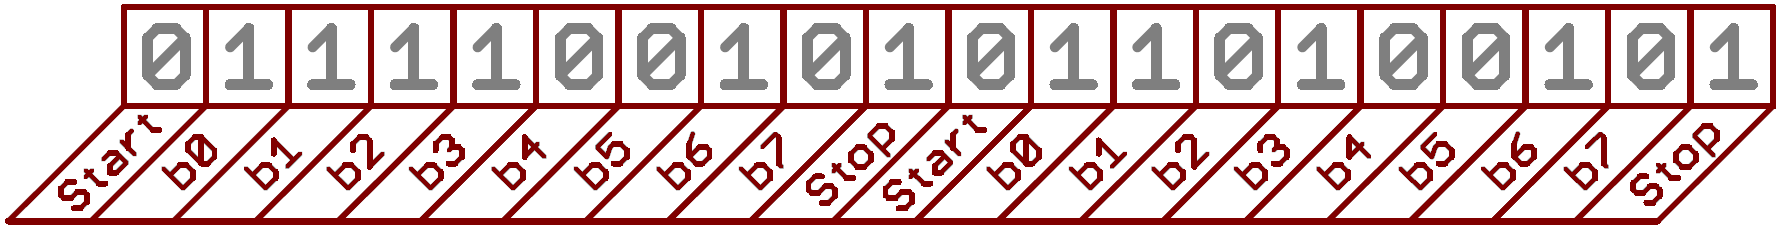
\includegraphics[scale=0.3]{Pictures/uart_ok.png}
        \caption{\textit{Nachricht 'OK' \citep{ImgRXTX}}}
        \label{img:uart_ok}
\end{figure}

Die Bitfolge '01001111' entspricht dem Buchstaben 'O', die Bitfolge '01001011' die dem Buchstaben 'K'.



\subsubsection{MQTT} 

MQTT ist ein simples Client-Server-Protokoll zur Nachrichtenübertragung, häufig genutzt in \ac{IoT}-Anwendungen oder im industriellen Umfeld. Durch
die geringe Belegung von Bandbreite eignet es sich in Netzwerken mit hoher Latenz, schlechten Verbindungen und zur Nutzung auf Geräten
mit vergleichsweise geringer Rechenleistung \citep{MQTT_FAQ}.

\smallskip

Geräte, welche Daten empfangen oder versenden (s.g. Clients) sind mit einem zentralem Server (s.g. Broker) verbunden. Nach erfolgreicher Verbindung
der Clients mit dem Broker versenden diese ihre Nachrichten mit einem s.g. Topic, welches die versendete Nachricht hierarchisch einstuft.
Ein Beispiel wäre zum Beispiel \lstinline!Hochschule/B/Temp!. Sendet nun ein Client eine Nachricht mit diesem Topic, wird 
diese Nachricht an alle Clients weitergeleitet, welche dieses Topic abonniert haben. Diese Art der Kommunikation wird Publish/Subscribe-Modell 
genannt \citep{MQTT_Article} und wird in Abb. \ref{img:MQTT} dargestellt. 

\begin{figure}[h]
    \vspace{-\baselineskip}
        \centering
        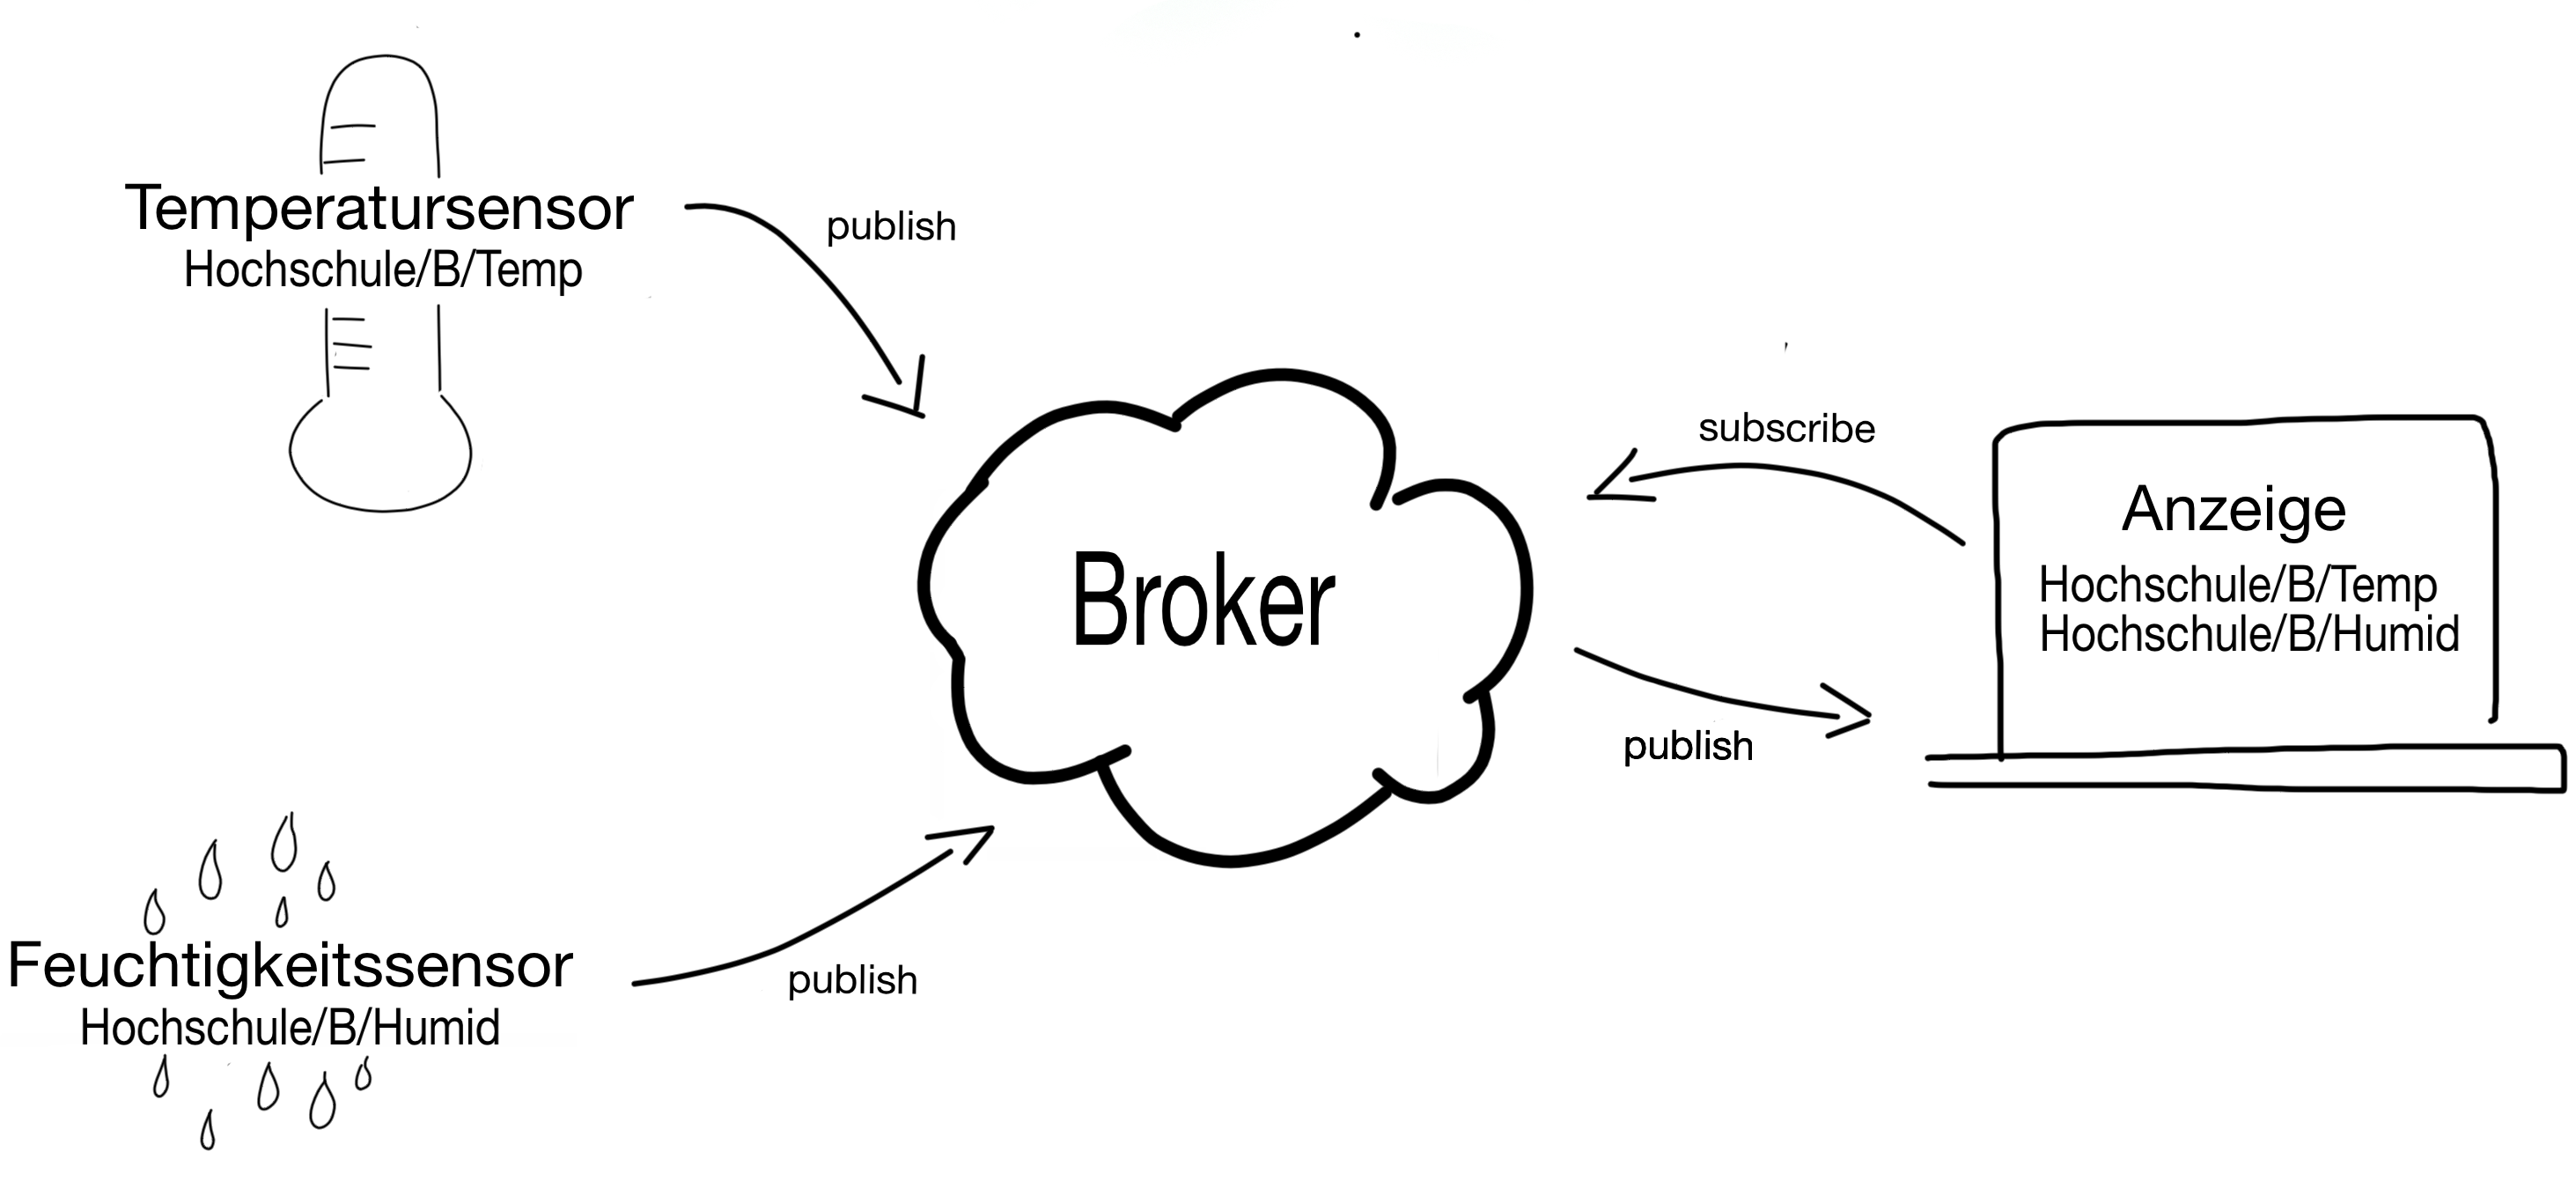
\includegraphics[scale=0.5]{Pictures/brokerclient.png}
        \caption{\textit{Publish/Subscribe-Modell}}
        \label{img:MQTT}
\end{figure}

\smallskip

MQTT besitzt diverse Features, welche, abgesehen von der Simplizität, attraktiv für den Einsatz im industriellen Umfeld sind \citep{MQTT_Article}:

\paragraph{Quality of Service Level}
Durch den Quality of Service Level kann sichergestellt werden, dass eine Nachricht beim Empfänger ankommt, auch wenn es zu Verbindungsabbrüchen kommt.
\paragraph{Retained Messages}
Die letzte gesendete Nachricht eines Topics wird im Broker hinterlegt. Verbindet sich ein neuer Client mit diesem Topic, erhält er automatisch
die gespeicherte Nachricht.
\paragraph{Last Will and Testament}
Sobald der Broker feststellt, dass ein Client die Verbindung ohne eine Abmeldung verloren hat, wird eine Nachricht an alle Clients, welche das
selbe Topic abonniert haben, versendet.
\paragraph{Persistent Sessions}
Falls mit häufigen Verbindungsabbrüchen zu rechnen ist, kann der Broker alle durch einen Verbindungsabbruch verpasste Nachrichten automatisch 
erneut an den Client versenden.



\clearpage
\subsection{Datenstrukturen und Algorithmen}
\subsubsection{Ringbuffer}

\begin{wrapfigure}{r}{0.45\textwidth}
    % \begin{figure}[h]
     \vspace{-\baselineskip}
         \centering
         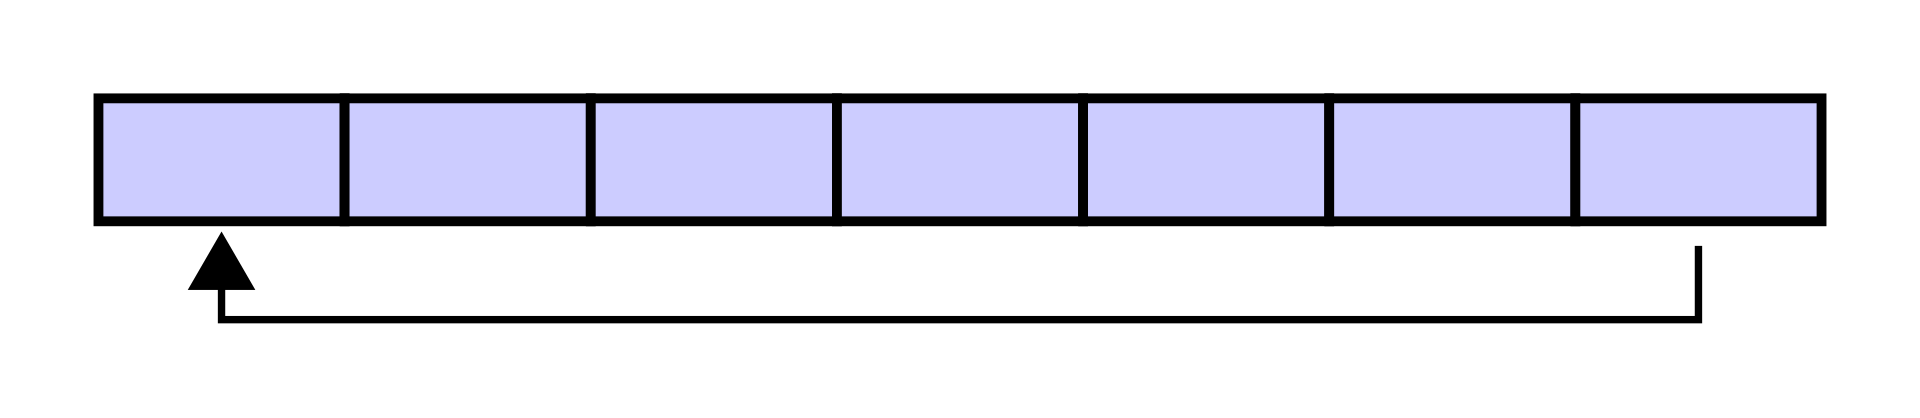
\includegraphics[scale=0.1]{Pictures/circular_buffer.png}
         \caption{\textit{Ringbuffer \citep{ImgBuffer}}}
         \label{img:Ringbuffer}
    % \end{figure}
 \end{wrapfigure}

Der Ringbuffer ist eine Datenstruktur welche nach dem \acs{FIFO}-Prinzip arbeitet. Dies bedeutet, dass die Daten, welche
zuerst in den Buffer geschrieben wurden, auch zuerst wieder ausgelesen werden. 

\smallskip

Die zu schreibenden Daten werden in ein Array von bestimmter Länge N geschrieben. Läuft das Array voll, werden die neuen Zeichen
wieder an den Anfang geschrieben. Zur Orientierung werden zwei Zähler eingeführt, der s.g. Lese- und Schreibindex. Der Leseindex
zeigt die aktuelle Position im Array an, an der gelesen wird, während der Schreibindex anzeigt, bis an welche Stelle
neue Daten geschrieben wurden.  

Haben Lese- und Schreibindex den selben Wert, wird der Buffer als leer angesehen. 

\smallskip

Wird ein Zeichen in den Ringbuffer geschrieben, wird der Schreibindex inkrementiert. Sobald ein Zeichen gelesen wird, wird der Leseindex
inkrementiert. Erreichen die beiden Indexe das Ende des Arrays, werden sie auf null zurückgesetzt.


\subsubsection{Zyklische Redundanzprüfung}

Die Zyklische Redundanzprüfung, im englischen \textit{cyclic redundancy check} genannt, kurz \textbf{CRC} ist eine Methode zur Erkennung von Fehlern bei 
der Übertragung. Es ist nur möglich, zufällige Fehler zu erkennen, wie sie z.B. durch Übertragungsfehler oder Rauschen auf der Leitung entstehen \citep{IK_VL}.

\smallskip

Den zu übertragenden Daten wird ein zuvor berechneter Wert angehängt. Mittels dieses Wertes kann nun die Empfängerseite feststellen, ob die Daten korrekt übertragenden
wurden, oder ob ein Fehler vorliegt. 

\smallskip

CRC nutzt zur Überprüfung der Daten die Polynomdivsion. Die Daten, welche übertragen werden sollen, werden als Polynom dargestellt.

\smallskip

Die Bitfolge \begin{math}
    10101010
\end{math}  entspricht dem Polynom \begin{math}
    1*x^7+0*x^6+1*x^5+0*x^4+1*x^3+0*x^2+1*x+0
\end{math}.
Das Polynom der Bitfolge wird durch ein zuvor festgelegtes CRC-Polynom geteilt. Der Rest dieser mathematischen Operation repräsentiert den CRC-Wert. Dieser Wert
wird anschließend bei der Datenübertragung an die zu übertragende Nachricht angehängt.

\smallskip

Empfängerseitig wird nun abermals eine Polynomdivision durchgeführt. Ist das Ergebnis der Polynomdivision empfangene Nachricht inkl. CRC-Wert dividiert durch das
CRC-Polynom gleich null, wurde die Nachricht korrekt übertragen \citep{IK_VL}.


\subsection{STM32 Hardware Abstraction Layer und CubeMX}

Der \ac{HAL} ist eine Schnittstelle zwischen der untersten Firmwareschicht des STM32 und der Software, welche der Nutzer schreibt. Durch die Benutzung des
\acp{HAL} müssen keine einzelnen Register mittels Assembler gesetzt werden. Die Konfiguration wird dadurch stark vereinfacht und die Fehleranfälligkeit verringert.

\smallskip

Die dazu notwendigen Libraries werden vom Hersteller (ST) bereitgestellt und dokumentiert \citep{HAL_Description}. 

\smallskip

Funktionen, welche vom \ac{HAL} bereitgestellt werden, sind zu erkennen an einem vorgestellten \textit{HAL}. Folgende Funktion schaltet z.B. einen \ac{GPIO} um:

\smallskip

\begin{lstlisting}
    HAL_GPIO_TogglePin(GPIOx, GPIO_Pin);
\end{lstlisting}

\smallskip

Neben dem \ac{HAL} stellt der Hersteller ein weiteres Tool zur Verfügung (Cube MX \citep{CubeMX}), welche die schnelle Erstellung des Initialiserungscodes 
für die Peripherie und sonstige Funktionen ermöglicht. Dies verringert ebenfalls die Fehleranfälligkeit und vereinfacht die Programmierung.

Mittels einer graphischen Oberfläche können den verschieden Anschlüssen des \ac{uC} Funktionen zugewiesen (z.B. \ac{I2C}) werden und die Timings und Taktfrequenzen
konfiguriert werden.

\vspace{0.5cm}

\begin{figure}[h]
    \vspace{-\baselineskip}
        \centering
        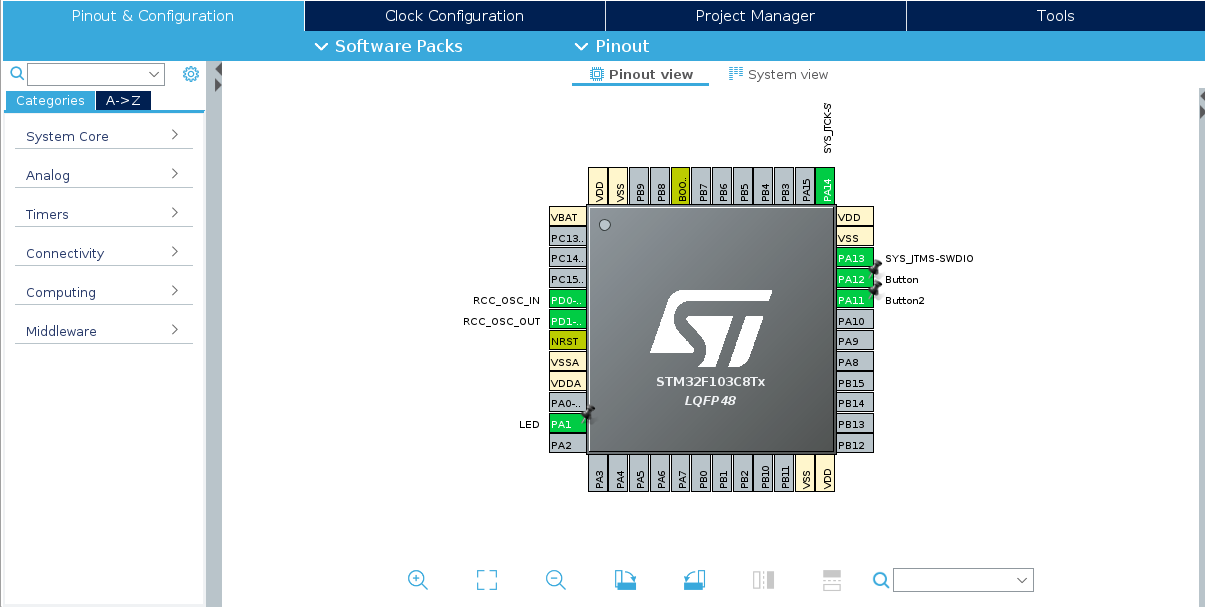
\includegraphics[scale=0.3]{Pictures/cubeMX.png}
        \caption{\textit{CubeMX}}
        \label{img:CubeMX}
\end{figure}
\clearpage

\section{Umsetzung}
\label{sec:Umsetzung}
\subsection{Protokoll}

Im folgenden soll die Entwicklung des Protokolls erklärt werden. Zuerst wird auf den Algorithmus zur zyklischen Redundanzprüfung eingegangen,
anschließend auf den Aufbau der übertragenen Nachrichten.

\subsubsection{CRC16-CCITT}

Als Implementation der zyklische Redundanzprüfung wurde die Version \textit{CRC16-CCITT} gewählt, da diese bewährt und gut dokumentiert ist. Leider 
kursieren viele fehlerhafte Implementationen dieses Algorithmus - es wurde jedoch wert darauf gelegt, die Richtige Version zu implementieren.

\smallskip

Das CRC-Polynom lautet $x^{16}+x^{15}+x^2+1$. Die hexadezimale Repräsentation ergibt sich deshalb zu $0x1021$.
\smallskip

Als Startwert für die Berechnung wird $0x0$ gewählt - fehlerhafte Implementationen beginnen oftmal mit $0xFFFF$. 

\begin{wraptable}{l}{30mm} 
    \centering
\begin{tabular}{ |c | c | c | }
    \hline
    a & b & y \\
    \hline \hline
    0 & 0 & 0 \\
    \hline
    0 & 1 & 1 \\
    \hline
    1 & 0 & 1 \\
    \hline
    1 & 1 & 0 \\
    \hline
\end{tabular}
\caption{XOR}
\end{wraptable}

\smallskip

Zwar handelt es sich bei der Berechnung des CRC-Wertes um eine Division, allerdings um eine \textit{Polynom}divsion - diese wird mit Hilfe eines Exklusiv-Oder
Gatters (\textit{XOR}) und Schieberegistern realisiert. Den zu prüfenden Daten werden abhängig von der Länge des CRC-Polynoms Nullen angehängt, in diesem Falle also 
16 Stück.

\smallskip

Um die Daten zu Prüfen, wird das CRC-Schieberegister mit '0' initialisiert. Anschließend wird der zu prüfende Wert, mit angehängten Nullen von rechts
in das Schieberegister "geschoben", bis das \ac{MSB} gleich '1' ist. Anschließend wird das Schieberegister um eine Einheit weitergeschoben, sodass das \ac{MSB}
herausfällt. Dann wird das Schieberegister mit Hilfe des XOR-Vergleiches mit dem CRC-Polynom verglichen. Der so entstandene Wert wird wieder in das Schieberegister
übernommen \citep{IK_VL}. 

\smallskip

Nun werden immer wieder Daten von rechts in das Register hineingeschoben. Immer wenn das \ac{MSB} einer '1' entspricht und im nächsten Schritt aus dem Register
geschoben wird, wird ein XOR-Vergleich mit dem CRC-Polynom durchgeführt. Dies wird so lange wiederholt, bis keine neuen Daten mehr in das Register geschoben werden können.
Der Wert welcher nun im Schieberegister verbleibt, entspricht der Prüfsumme \citep{IK_VL}.

\smallskip

Die Implementation in C bedient sich zweier Kniffe, um die zuvor erklärte Berechnung zu beschleunigen. Auf ein Initialisieren mit 0x0000 kann verzichtet werden,
da keine XOR-Vergleiche mit Nullen durchgeführt werden. Der Startwert wird also direkt mit den Eingangsdaten initialisiert werden. Auch auf ein anhängen der Nullen 
kann verzichtet werden, da der \textit{<<-Operator (left shift)} automatisch am \ac{LSB} Nullen anhängt. 

\newpage

Umgesetzt in C Code entsteht folgende Funktion: 

\begin{lstlisting}[caption={\textit{Berechnung CRC16}}]
uint16_t CRC16_buf(const uint8_t * pBuf, uint16_t len) 
{
const uint16_t poly = 0x1021;
uint16_t crc = 0;

for (uint8_t i = 0; i < len; i++)
{
    crc ^= pBuf[i] << 8; //Move Byte into 16Bit CRC Register

    for(uint8_t j = 0; j < 8; j++)
    {
        if((crc & 0x8000) != 0) //Test for MSB
        {
            crc = (crc<<1) ^ poly; //If MSB = 1 shift & XOR
        }
        else
            crc <<= 1;	//If not just shift
    }
}
return crc;
}
\end{lstlisting}

Der Funktion wird ein Zeiger zu einem Array übergeben, sowie die Länge dieses Arrays. Die Variable \lstinline!poly! repräsentiert das CRC-Polynom,
während die Variable \lstinline!crc! für das Schieberegister steht.

\smallskip

Die Berechnung des CRC-Wertes wird für jedes Byte des Arrays durchgeführt, wobei der Startwert für jedes Byte nach dem ersten die CRC-Prüfsumme des 
letzten Durchlaufes ist. Für jedes Byte wiederrum müssen, auf Grund der länge eines Bytes, acht mal die Shift- und XOR-Operationen durchgeführt werden.

\smallskip

Mittels des Wertes \lstinline!0x8000! wird geprüft, ob das \ac{MSB} gesetzt ist. Der Rückgabewert entspricht der CRC-Prüfsumme. 

\newpage

\subsubsection{Datenformat}
\label{subsub: Datenformat}

Bei den übertragenen Daten handelt es sich um Zeichen im \acs{ASCII}-Format. Dies vereinfacht die Auswertung und hat den Vorteil, dass die Kommunikation
zu Testzwecken leicht mitgelesen werden kann. Im folgenden wird unter \textit{Telegramm} die Gesamtheit der übertragenen Daten verstanden, während 
der Ausdruck \textit{Nachricht} den eigentlichen Informationsgehalt beschreibt.

\smallskip

Ein Telegramm teilt sich in mehrere Teile auf:

\begin{itemize}
    \item Startzeichen
    \item Länge
    \item Nachricht
    \item CRC-Prüfsumme
\end{itemize}



Die verschiedenen Teile bestehen aus einer verschiedenen Anzahl an Bytes. Während Start- und Endzeichen nur ein Byte benötigen, werden für die
Länge der Nachricht und die CRC-Prüfsumme zwei Bytes benötigt.

\smallskip

\begin{wraptable}{r}{75mm} 
    
    \begin{tabular}{ |c | c | c | c | c | c | c | }
        \hline
        1 & 2 & 3 & 4 & n+4 & n+5 & n+6  \\
        \hline \hline
        Start  & \multicolumn{2}{|c|}{Länge} & \multicolumn{2}{|c|}{Nachricht} & \multicolumn{2}{|c|}{CRC16} \\
        \hline
    
      \end{tabular}
    \centering
    \caption{Telegramm}
    \end{wraptable}


Da die Länge der Nachricht aus zwei Bytes besteht, ergibt sich eine maximale Nachrichtenlänge von 99 Bytes. Auf ein Endzeichen wird verzichtet - 
das Ende des Telegramms berechnet sich aus der Länge der Nachricht. Das Startzeichen entspricht dem \acs{ASCII}-Zeichen '<'.

\subsubsection{Nachrichtentypen}
\label{subsub: Nachricht}

Basierend auf dem in \ref{subsub: Datenformat} beschriebenen Format werden nun verschiedene Nachrichtentypen implementiert, welche die Steuerung
der Platine ermöglichen oder der Information dienen. Dabei ist zu Unterscheiden, ob es sich um Nachrichten handelt, welche an das Board geschickt werden,
oder um Nachrichten, welche vom Board versendet werden.
Die Nachrichten werden dabei durch den STM32 verarbeitet, der ESP8266 leitet sie weiter. 

\smallskip

Um die Nachrichten zu differenzieren, wird bei Nachrichten welche an das Board gesendet werden die Nachricht durch eine \ac{ASCII}-Zahl 
kodiert, bei Nachrichten welche das Board sendet durch einen \ac{ASCII}-Buchstaben.

\smallskip

\underline{Nachrichten in Senderichtung:}
\begin{itemize}
    \item STATUS (1) - Abfrage der Versionsnummer, genutzter Sensor
    \item CALIBRATE (2) - Kalibrieren des Sensors
    \item SENDVAL (3) - Start der automatischen Versendung von Messwerten 
\end{itemize}
Der Nachricht SENDVAL wird desweiteren noch eine '1' oder eine '0' angehängt, um die Funktion ein- oder auszuschalten.

\smallskip

Soll nun z.B. der Status des Boards abgefragt werden, wird die Nachricht STATUS versendet. Diese Nachricht ist genau 1 Byte lang, deshalb
wird als Längeninformation die \ac{ASCII}-Zahlen '0' und '1' übertragen. Danach folgt die eigentliche Nachricht, welche ebenfalls durch eine '1' 
repräsentiert wird. Abgeschlossen wird das Telegramm durch die CRC-Prüfsumme. Das Telegramm ergibt sich somit zu:

\begin{table}[h]
\centering
\begin{tabular}{| c | c | c | c | c | c | c |}
    \hline
    \textbf{Zeichen} & 1 & 2 & 3 & 4 & 5 & 6 \\
    \hline \hline
    \textbf{ASCII} & < & 0 & 1 & 1 & \multicolumn{2}{|c|}{CRC16} \\
    \hline \hline
    \textbf{Hex} & 0x3C & 0x30 & 0x31 & 0x31 & 0xB6 & 0xA8 \\
    \hline
    
\end{tabular}
\caption{SENDVAL}
\end{table}

\underline{Nachrichten in Empfangsrichtung:}
\begin{itemize}
    \item BOARD (B) - Antwort auf STATUS, enthält zusätzlich Versionsnummer und Sensortyp
    \item ANVALUE (A) - Zeigt einen Messwert an
    \item ERROR (E) - Zeigt einen Fehler an, gefolgt vom Errortyp
    \item ACK (A) - Acknowledge, automatische Antwort auf empfangene Nachrichten
\end{itemize}

Die Nachricht ACK gibt den empfangenen Nachrichtentyp zurück, um sicherzugehen, dass die gesendete Nachricht korrekt empfangen wurde.
Dem Nachrichtentyp ERROR folgt immer der Typ des aufgetretenen Fehlers, repräsentiert durch eine Zahl:

\begin{itemize}
    \item ER\_UNSPEC (1) - unspezifizierter Error
    \item ER\_CAL (2) - Fehler bei der Kalibrierung des Sensors
    \item ER\_NOT\_CAL (3) - Sensor nicht Kalibriert
    \item ER\_UN\_MSG (4) - Die empfangene Nachricht kann nicht interpretiert werden
\end{itemize}
\clearpage
\subsection{Empfang von Daten}

Die Daten müssen auf beiden \ac{uC} ordnungsgemäß empfangen werden. Die Implementation unterscheidet sich hierbei stark. Der STM32 ermöglicht
die Nutzung seiner \ac{DMA}-Funktionalität, während auf dem ESP8266 eine Interruptbasierte Abfrage implementiert wird.

\subsubsection{STM32: Strukturvariable DMA\_STRUCT}

Aus Gründen der Übersichtlichkeit wurde für die Datenverarbeitung des STM32 eine Strukturvariable definiert, welche hiermit eingeführt wird.
Die Strukturvariable \lstinline!DMA_STRUCT! enthält mehrere weitere Variablen für Flags und Zähler.

\begin{lstlisting}[caption={\textit{DMA Strukturvariable}}]
typedef struct
{
    volatile uint8_t  t_flag;   
    uint8_t tx_flag;			
    uint16_t timer;             
    uint16_t prevCOUNT;         
} DMA_STRUCT;
\end{lstlisting}

Die Flags \lstinline!t_flag! und \lstinline!tx_flag! dienen der Identifikation von Interrupts, welche durch im Falle von \lstinline!t_flag! durch ein
Timeout ausgelöst wurden oder im Falle von \lstinline!tx_flag! durch das erfolgreiche Senden von Daten. Die Variable \lstinline!timer! legt 
die Zeitkonstante für den Timeout fest, während \lstinline!prevCOUNT! einen Zähler speichert, der in \ref{subsub: Empfang} genauer erklärt wird.   

\subsubsection{STM32: Konfiguration des UART}
Wichtig bei der Konfiguration des \acp{UART} ist das Format und die Baudrate. Wie in \ref{sec:Grundlagen} erklärt, wird der \ac{UART} im 8N1-Modus
konfiguriert. Dies entspricht einer Nachrichtenlänge von acht Bit und keiner Parität. Die Geschwindigkeit wird auf 115200 Baud festgelegt (siehe Abb. \ref{img: Parameter}). 

\smallskip

Um die Nutzung des \ac{UART} in Kombination mit \ac{DMA} zu ermöglichen, muss der globale Interrupt
aktiviert werden. Der \ac{DMA} wird so konfiguriert, dass empfangsseitig die Daten direkt zum Speicher übertragen werden, während senderseitig die Daten
direkt vom Speicher zum \ac{UART} weitergeleitet werden. Zudem wird der Empfang von Daten per \ac{DMA} als Ringbuffer umgesetzt (siehe Abb. \ref{img: DMA}).


\begin{figure}[h]
    \centering
    \begin{subfigure}{0.45\textwidth}
        \centering
        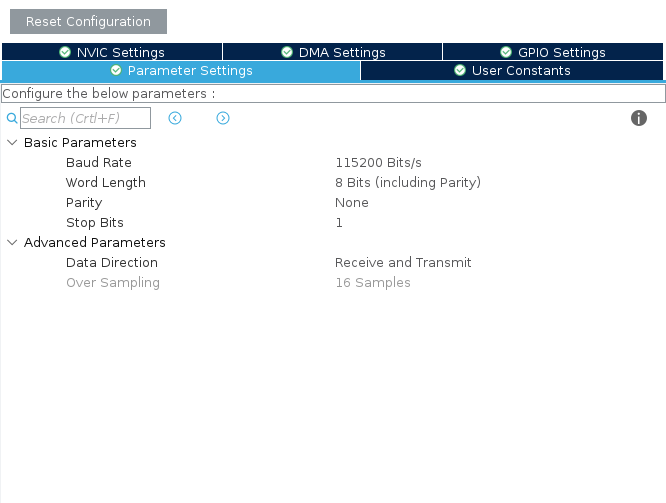
\includegraphics[width=\textwidth]{Pictures/parameter_uart.png}
        \caption{Baudrate,Format}
        \label{img: Parameter}
    \end{subfigure}
    %
    \begin{subfigure}{0.45\textwidth}
        \centering
        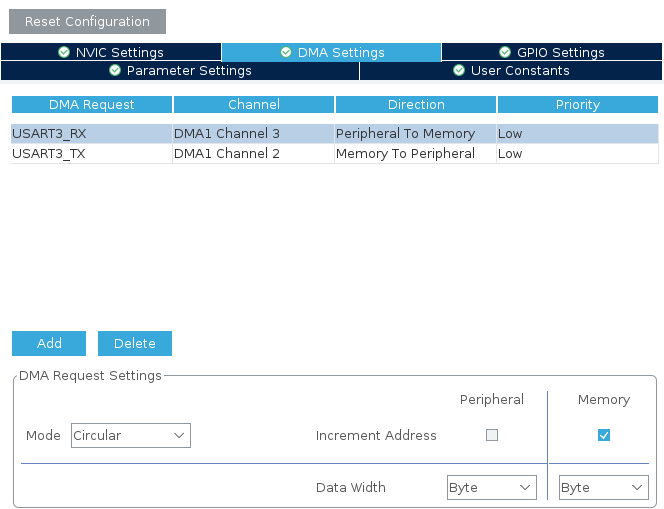
\includegraphics[width=\textwidth]{Pictures/dma_uart.png}
        \caption{DMA}
        \label{img: DMA}
    \end{subfigure}
    \caption{Konfiguration des \acp{UART}}
    \label{img: UART config}
  \end{figure}

  \subsubsection{STM32: Idle Line Detection}
  \label{subsub: Idle}

  Es ist von großem Vorteil, zu erkennen, wenn keine Daten mehr Empfangen werden, um das schreiben von sinnlosen Daten in den Buffer zu vermeiden.
  Deshalb wird eine s.g. \textit{Idle Line Detection} implementiert, welche erkennt, sobald keine Daten mehr empfangen werden.

  \newpage

  Der STM32 bietet dafür einen Interrupt, welcher manuell aktiviert werden muss \citep{STM32_Ref}. Um den Interrupt zu aktivieren, muss in der Datei
  \lstinline!stm32f1xx_it.c! die Funktion 
  
  \lstinline!void USARTX_IRQHandler(void)! folgendermaßen erweitert werden:

  \begin{lstlisting}[caption={\textit{Idle Line Interrupt}}]
    if(__HAL_UART_GET_FLAG(&huartx,UART_FLAG_IDLE))
    {
        __HAL_UART_CLEAR_IDLEFLAG(&huartx);
        dma_info.timer = DMA_TIMEOUT_MS;
    }
  \end{lstlisting}

  Jedes mal, wenn ein Interrupt in Zusammenhang mit dem \ac{UART} ausgelöst wird, wird die Routine \lstinline!void USARTX_IRQHandler(void)! 
  aufgerufen  und geprüft, ob es sich um ein Idle Line Interrupt handelt \citep{STM32_Ref}. 

  \smallskip

  Es ist allerdings nicht ausreichend, nur zu prüfen, ob der Interrupt aufgetreten ist - es kann durchaus vorkommen, dass es sich nur um eine
  kurze Unterbrechung in der Kommunikation handelt. Deshalb wird die Funktionalität um einen Timeout erweitert. Wenn der Interrupt auftritt, wird
  gleichzeitig die Strukturvariable \lstinline!dma_info.timer! mit einer definierten Zeitwert \lstinline!DMA_TIMEOUT_MS! geladen.

  \smallskip

  Um für zukünftige Erweiterungen keinen Timer zu blockieren, wird für den Timeout der Systick-Timer (\ref{subsub: Timer}) genutzt. Dieser implementiert eine Routine,
  welche im 10ms-Takt aufgerufen wird. Diese Routine ist ebenfalls in der Datei \lstinline!stm32fxx_it.c! zu finden und wird um folgenden Code
  erweitert:

  \begin{lstlisting}[caption={\textit{Systick Timer}}]
    if(dma_info.timer == 1)
    {
        dma_info.t_flag = 1;
        HAL_UART_RxCpltCallback(&huartx);
    }
    if(dma_info.timer) 
    { 
        --dma_info.timer; 
    }



  \end{lstlisting}
  
  Mittels dieser Erweiterung wird nun immer der Zähler des Timeouts dekrementiert, bis er eins erreicht. Wenn dies geschieht, wird ein Flag gesetzt
  und die Interruptroutine \lstinline!HAL\_UART\_RxCpltCallback(&huartx)! aufgerufen, in welcher anschließend der aufgetauchte Interrupt mittels des
  gesetzten Flags identifiziert und verarbeitet wird.
  
  \subsubsection{STM32: Empfangsinterrupt / DMA Circular Buffer}
  \label{subsub: Empfang}

  Während der Kommunikation mit \ac{UART} werden verschiedene Interrupts ausgelöst. Bei der Nutzung von \ac{DMA} werden Interrupts ausgelöst,
  wenn der Buffer halb oder ganz voll ist \citep{STM32_Ref}. Desweiteren wurde der \ac{uC} so konfiguriert, dass auch bei einem Idle Line Interrupt
  die entsprechende Interruptroutine aufgerufen wird \ref{subsub: Idle}.

  \smallskip

  Die Interruptroutinen sind nach der Generation von Code mittels CubeMX in der Datei \lstinline!stm32f1xx_hal.c! als \lstinline!__weak!
  definiert, werden also neu gesetzt sobald sie ohne das Keyword \lstinline!__weak! definiert werden \citep{HAL_Description}. 

  \smallskip

  In \lstinline!main.c! wird die Interruptroutine für den Empfang von Daten per \ac{UART} mit dem Namen 
  \begin{lstlisting}
    void HAL_UART_RxCpltCallback(UART_HandleTypeDef *huart)
  \end{lstlisting}
  initialisiert. 
  
  \smallskip

  Die Variablen \lstinline!pos!, \lstinline!start! und \lstinline!length! werden für den Ringbuffer benötigt. Die Variable \lstinline!currCount! speichert die aktuelle Position des
  Ringbuffers und wird über den Befehl
  
  \begin{lstlisting}
    __HAL_DMA_GET_COUNTER(huart->hdmarx)
  \end{lstlisting}
  beschrieben.

  \smallskip

  Die Variable \lstinline!start! enthält die Startposition, ab welcher neue Daten im Ringbuffer enthalten sind. In der Variable \lstinline!length!
  ist die Länge der Daten gespeichert. Tritt ein Interrupt auf, weil der Empfangsbuffer voll ist, berechnet sich die Länge der empfangenen 
  Daten simpel durch folgenden Befehl:
  \begin{lstlisting}
    length = DMA_BUF_SIZE - start;
  \end{lstlisting}
  Es kann nun jedoch dazu kommen, dass nachdem der Buffer voll ist, ein Timeout-Interrupt ausgelöst wird. Um nun falsche Verarbeitung von 
  Daten zu verhindern, wird die aktuelle Position des Buffers auf die Größe des Buffers gesetzt.
  \begin{lstlisting}
    dma_info.prevCOUNT = DMA_BUF_SIZE;      
  \end{lstlisting}

  \newpage
  
  Wird nun ein Timeout-Interrupt ausgelöst, wird die Routine durch folgenden Code frühzeitig abgebrochen und das Flag rückgesetzt:
  \begin{lstlisting}[caption={\textit{Abbruch Timeoutinterrupt}}]
    if(dma_info.t_flag && currCOUNT == DMA_BUF_SIZE)
    {
        dma_info.t_flag = 0;
        return;
    }
  \end{lstlisting}

  \smallskip

  Tritt ein Interrupt auf, weil ein Timeout aufgetreten ist, muss unterschieden werden ob im Buffer bereits alte Daten liegen, welche ignoriert
  werden müssen oder ob der Buffer mit zu verarbeitenden Daten gefüllt ist. Folgender Code implementiert dies:

  \begin{lstlisting}[caption={\textit{Längenberechnung Timeout}}]
    if(dma_info.t_flag)
    {
    	if(dma_info.prevCOUNT < DMA_BUF_SIZE)
    	{
    		length = dma_info.prevCOUNT - currCOUNT;
    	}
    	else
    	{
  		length = DMA_BUF_SIZE - currCOUNT;
  	}

        dma_info.prevCOUNT = currCOUNT;
        dma_info.t_flag = 0;
    }
  \end{lstlisting}

  Wenn ein Timeout-Flag aufgetreten ist, wird geprüft ob der alte Zähler des Ringbuffers kleiner als die Buffergröße ist. Ist dies der Fall, berechnet
  sich die Länge der Daten durch die Differenz zwischen dem alten und dem neuen Zählerwert, da noch alte Daten im Buffer gespeichert sind.
  
  Wenn keine alten Daten im Buffer gespeichert sind, berechnet sich die Länge durch die Differenz zwischen der Buffergröße und der aktuellen Zählerposition.

  \smallskip

  Im Anschluss wird der Zählerwert des \ac{DMA} übergeben und das Timeout-Flag rückgesetzt.

  \newpage

  Die Startposition der neuen Daten berechnet sich ähnlich. Ist der alte Zähler des Ringbuffers kleiner als die Buffergröße, ist die Startposition
  die Differenz zwischen der Buffergröße und des alten Zählerwerts. Wenn nicht, ist die Startposition gleich null.

  \begin{lstlisting}[caption={\textit{Berechnung Startposition}}]
    if(dma_info.prevCOUNT<DMA_BUF_SIZE)
    {
    	start = (DMA_BUF_SIZE-dma_info.prevCOUNT);
    }
    else
    {
    	start = 0;
    }  
  \end{lstlisting}

  \smallskip

  Mit Hilfe der berechneten Werten für die Startposition und die Länge der empfangenen Daten werden diese Daten zu guter Letzt in ein dediziertes
  Array zur Weiterverarbeitung kopiert und ein Flag gesetzt, welches anzeigt, dass neue Daten vorhanden sind:
  
  \begin{lstlisting}[caption={\textit{Kopieren neuer Daten}}]
    for(uint16_t i=0,pos=start; i<length; ++i,++pos)
    {
        data[i] = dma_rx_buf[pos];
    }
    data_avaiable = 1;
  \end{lstlisting}

  Mit den Informationen über das Protokoll aus \ref{subsub: Datenformat} lassen sich nun aus dem Array in dem die angekommenen Daten gespeichert wurden, die Telegramme extrahieren.

\subsubsection{STM32: Überprüfen der Daten}

Die empfangenen Daten müssen auf ihre Integrität getestet werden. Dazu wurde in \ref{subsub: CRC16} das Konzept der zyklischen Redundanzprüfung eingeführt.

\smallskip

Um die empfangenen Daten zu prüfen, wird das Array welches die Daten enthält der Funktion 
\begin{lstlisting}
  uint8_t data_check(uint8_t *dat)
\end{lstlisting}
übergeben. Diese Funktion extrahiert die CRC-Prüfsumme sowie die Länge der Nachricht und validiert diese. Wenn die zyklische Redundanzprüfung erfolgreich
ist, wird die Länge der Nachricht übergeben. Wenn sie fehlschlägt, wird eine null zurückgegeben.


\subsubsection{ESP8266: Empfang und Überprüfung der Daten}

Die Implementation für den Empfang von Daten 
\clearpage




%include list of figure
\listoffigures
\clearpage
\lstlistoflistings
\clearpage
%
%include list of tables
%\listoftables
%\clearpage

%Bibliotheksüberschrift anpassen
\bibliographystyle{unsrtnat} % plain, alpha, dinat
%Ändern der Überschrift des Literaturverzeichnisses zu Quellenverzeichnis
\renewcommand{\refname}{Quellenverzeichnis}
\bibliography{bibliography}


\clearpage





\mbox{}
\end{document}
